\documentclass[tikz,border=10pt]{standalone}
% Scale: 1 unit = 1/0.012739 px; origin at B; y flipped
\begin{document}
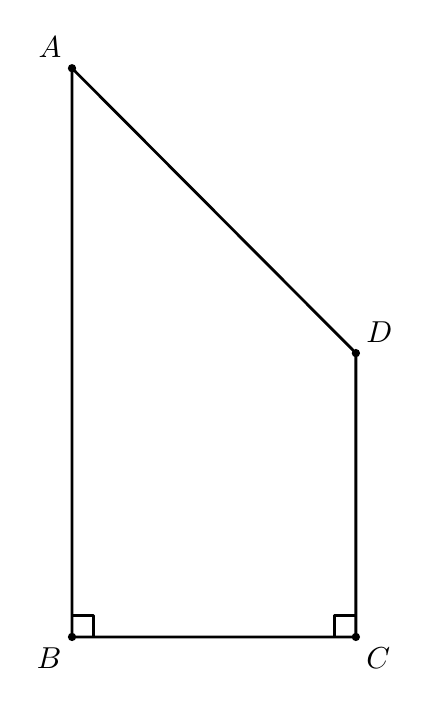
\begin{tikzpicture}[line join=round, line width=1.0pt]
  % Vertices (x = (px-69)*s, y = (632-py)*s)
  \coordinate (A) at (0,7.223);
  \coordinate (B) at (0,0);
  \coordinate (C) at (3.605,0);
  \coordinate (D) at (3.605,3.605);

  % Quadrilateral sides
  \draw (A) -- (B) -- (C) -- (D) -- cycle;

  % Right-angle marks at B and C (inside)
  \draw (0,0.27) -- (0.27,0.27) -- (0.27,0);
  \draw (3.335,0) -- (3.335,0.27) -- (3.605,0.27);

  % Vertex dots
  \fill (A) circle (1.5pt);
  \fill (B) circle (1.5pt);
  \fill (C) circle (1.5pt);
  \fill (D) circle (1.5pt);

  % Labels
  \node[above left] at (A) {\fontsize{10.5}{12.6}\selectfont $A$};
  \node[below left] at (B) {\fontsize{10.5}{12.6}\selectfont $B$};
  \node[below right] at (C) {\fontsize{10.5}{12.6}\selectfont $C$};
  \node[above right] at (D) {\fontsize{10.5}{12.6}\selectfont $D$};
\end{tikzpicture}
\end{document}